\documentclass[a4paper,12pt]{report}

\usepackage{alltt, fancyvrb, url}
\usepackage{graphicx}
\usepackage[utf8]{inputenc}
\usepackage{float}
\usepackage{xcolor}
\usepackage{hyperref}

\usepackage[italian]{babel}

\usepackage[italian]{cleveref}

\title{OOP24 - RUNWARRIOR}
\author{
    Samuele Bianchedi, Riccardo Cornacchia\\
    Francesca Gatti, Giovanni Maria Rava}
\date{\today}
\begin{document}
\maketitle
\tableofcontents
\chapter{Analisi}
\section{Descrizione e requisiti}
Il gruppo si pone come obbiettivo quello di realizzare una reinterpretazione del famoso gioco 
Super Mario Bross del 1986. Il gioco ha come personaggio principale un cavaliere, che tramite 
l'input dell'utente si muove in una mappa 2D. L'obbiettivo del cavaliere è salvare una princessa tenuta
prigioniera da uno stregone, completando diversi livelli che lo condurranno al castello nel quale è 
rinchiusa. Nel gioco sarà possibile, tramite un negozio, comprare un altro personaggio, se si ha raccolto un numero sufficiente di monete.
All'interno del gioco, oltre a diversi ostacoli, sono presenti nemici che il cavaliere può uccidere per rimanere in vita e 
completare il livello. 
\subsection*{Requisiti funzionali}
\begin{itemize}
    \item Il personaggio deve avanzare, indietreggiare e saltare all'interno della mappa.
    \item Gestione delle collisioni del personaggio con nemici, ostacoli, monete e potenziamenti.
    \item Il personaggio può ottenere due potenziamenti che lo aiuteranno nella sua avventura.
    \item Gestione di nemici ed ostacoli diversi in base alla mappa.
    \item Creazione di un sistema di punteggio, che verrà mostrato al completamento del livello.
\end{itemize}
\newpage
\subsection*{Requisiti non funzionali}
\begin{itemize}
    \item Implementazioni di una quarta mappa. 
    \item Gestione di restart e checkpoint.
    \item Creazione di nemici e ostacoli più complessi.
    \item Musica e suoni. 
\end{itemize}
\section{Modello del Dominio}
RunWarrior è gioco ambientato in un mondo fantastico in cui il personaggio principale deve affrontare 3 livelli diversi, selezionabili mediante un menù.
In questi livelli il personaggio deve portersi muovere per sopravvivere e uccidere i nemici. Il movimento del personaggio è gestito tramite tastiera.
All'interno della mappa sono posizionate delle uova che racchiudono al loro interno i 2 possibili powerup, diversi per Warrior e Wizard.
Per il completamento del gioco è neccessario sbloccare tutti i livelli in maniera sequenziale, che si considerano terminati 
tramite l'ingresso in un portale, ad eccezione del terzo che si conclude con il castello della principessa.
All'interno di ogni livello possono essere presenti degli ostacoli letali (MapElement) e dei nemici (Enemy) e delle monete (Coin) con il quale il 
personaggio può collidere. Se ciò accade con un ostacolo o con un nemico perde un potenziamento, nel caso lo avesse, altrimenti la partita finisce.
I nemici sono di 5 tipi:
\begin{itemize}
    \item Goblin
    \item Snake
    \item Wizard
    \item Monkey 
    \item Guard
\end{itemize}
Gli ostacoli letali sono:
\begin{itemize}
    \item Fungo
    \item Cactus
    \item Camino con fuoco
\end{itemize}

\begin{figure}
    \centering
    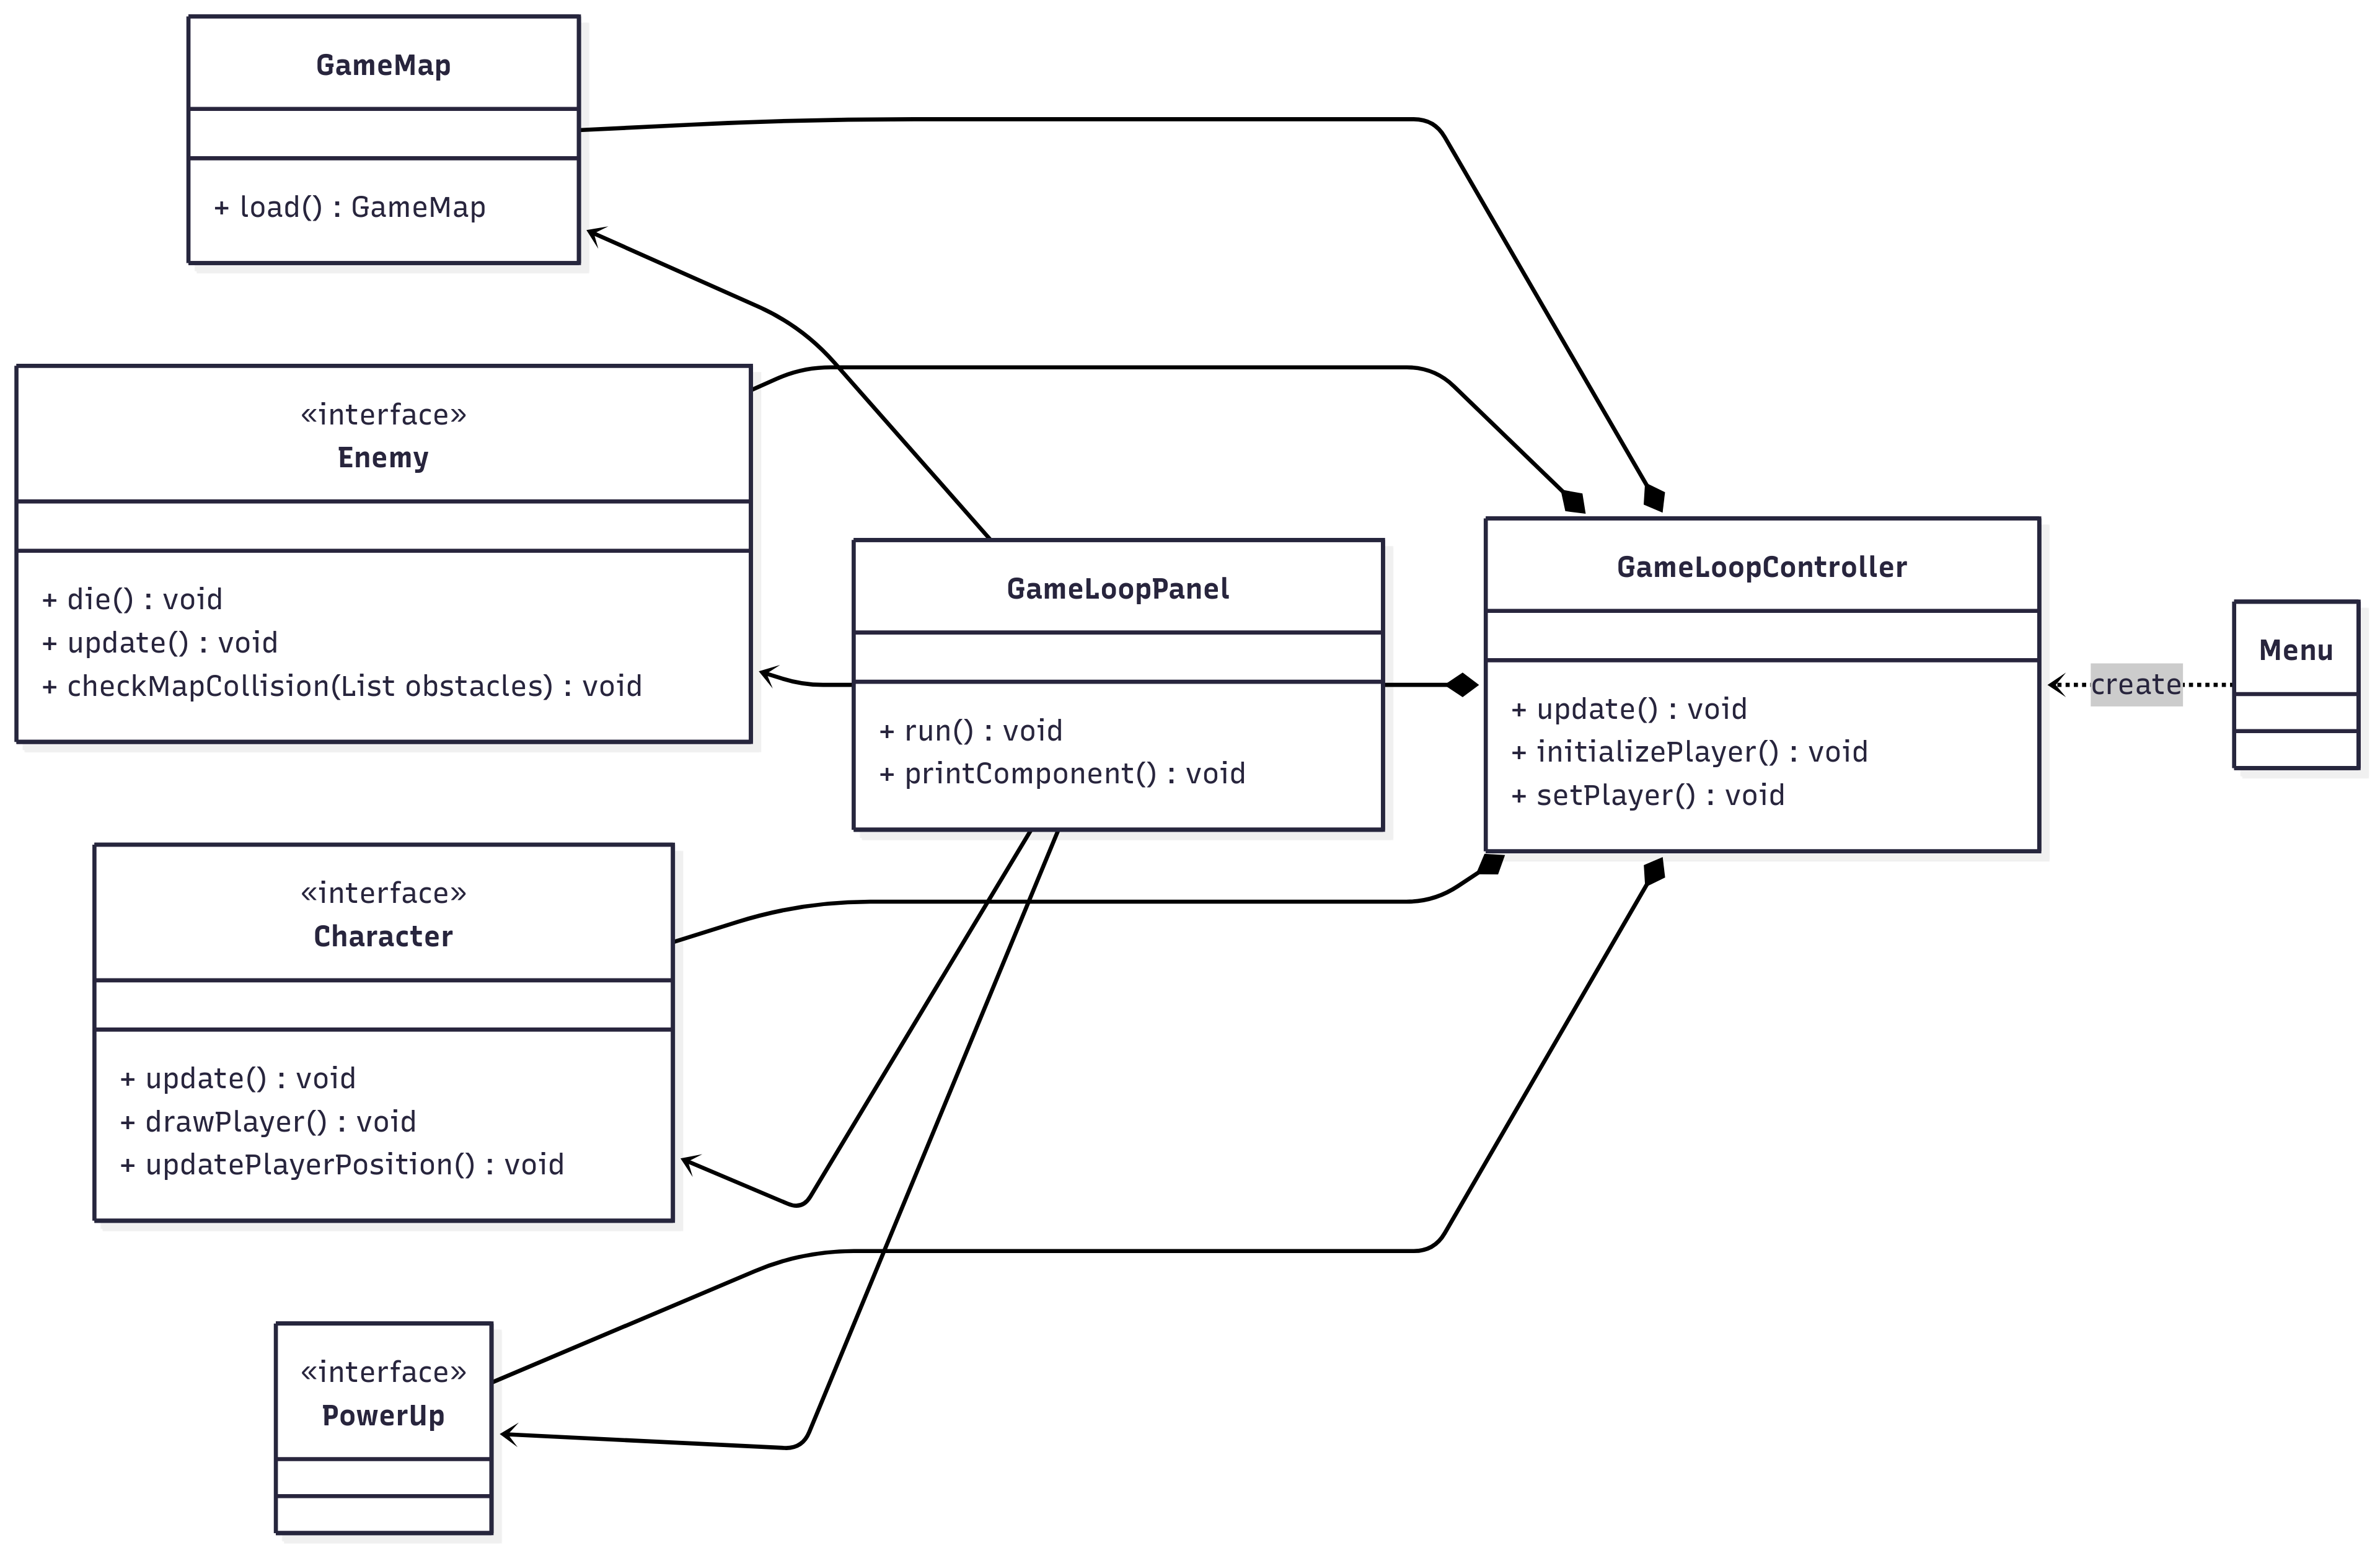
\includegraphics[width=\textwidth]{resources/modelloDominioUML.png}
    \caption{UML del modello del dominio}
    \label{}
\end{figure}
\chapter{Design}
\section{Architettura}
L'architettura di RunWarrior segue il pattern architetturale MVC (Model - View - Controller). Il GameLoopController gestisce l'aggiornamento
del gioco e di tutte le sue entità a seguito dei diversi eventi che possono capitare durante la sessione. All'interno della classe, 
dal momento in cui viene acquistato il nuovo personaggio, ricevendo le informazione da GameSaveManager e Shop, viene gestito il cambio skin.
Gli input da tastiera per muovere il personaggio vengono gestiti tramite la comunicazione tra le classi CharacterComand e MovementHandlerImpl.
Quindi il Character è una entità reattiva che modifica il proprio stato a seguito delle diverse collisioni con le entità, 
tramite CollisionDetection, KillDetection e PowerUpDetection.
Il pattern MVC implementato consente di mantenere lo stato del controller nell'eventualità che si modifichi la view.
inserire UML delle classi principali dell'MVC
\section{Samuele Bianchedi}
\textbf{Problema}: L'implementazioni delle classi del modello soffriva di una criticità legata all'incapsulamento. SptoBugs ha rilevato molti warning che indicavano oggetti mutabili passati e restituiti tramite riferimento diretto.
Questo poteva creare un’architettura fragile, incline ad errori e/o modifiche involontarie.
\textbf{Soluzione}: Per risolvere questo problema e rendere sicuro i dati ho scelto di implementare copie difensive.
\begin{itemize}
    \item Per oggetti come BufferedImage e int[][]: nei costruttori e nei metodi setter invece di memorizzare il riferimento all'oggetto, 
    ne viene creata una copia completa.
    \item Nei metodi getter: invece di restituire una riferimento all'oggetti ne viene creato uno nuovo da passare al chiamante
    \item Per le collezioni: i metodi getter sono stati modificato per restituire una vista immodificabile della collezione.
\end{itemize}
I pro sono ovviamente la sicurezza dei dati che sono protetti da modifiche esterne. Di contro abbiamo una riduzione della performance, 
in quanto copiare oggetti innumerevoli volte costa abbastanza e in alcuni casi ha portato a “freeze” dell'applicazione.
Nel seguente schema UML si mostra come i campi siano privati e l'accesso avvenga tramite metodi pubblici che lavorano restituendo copie.
\begin{figure}
    \centering
    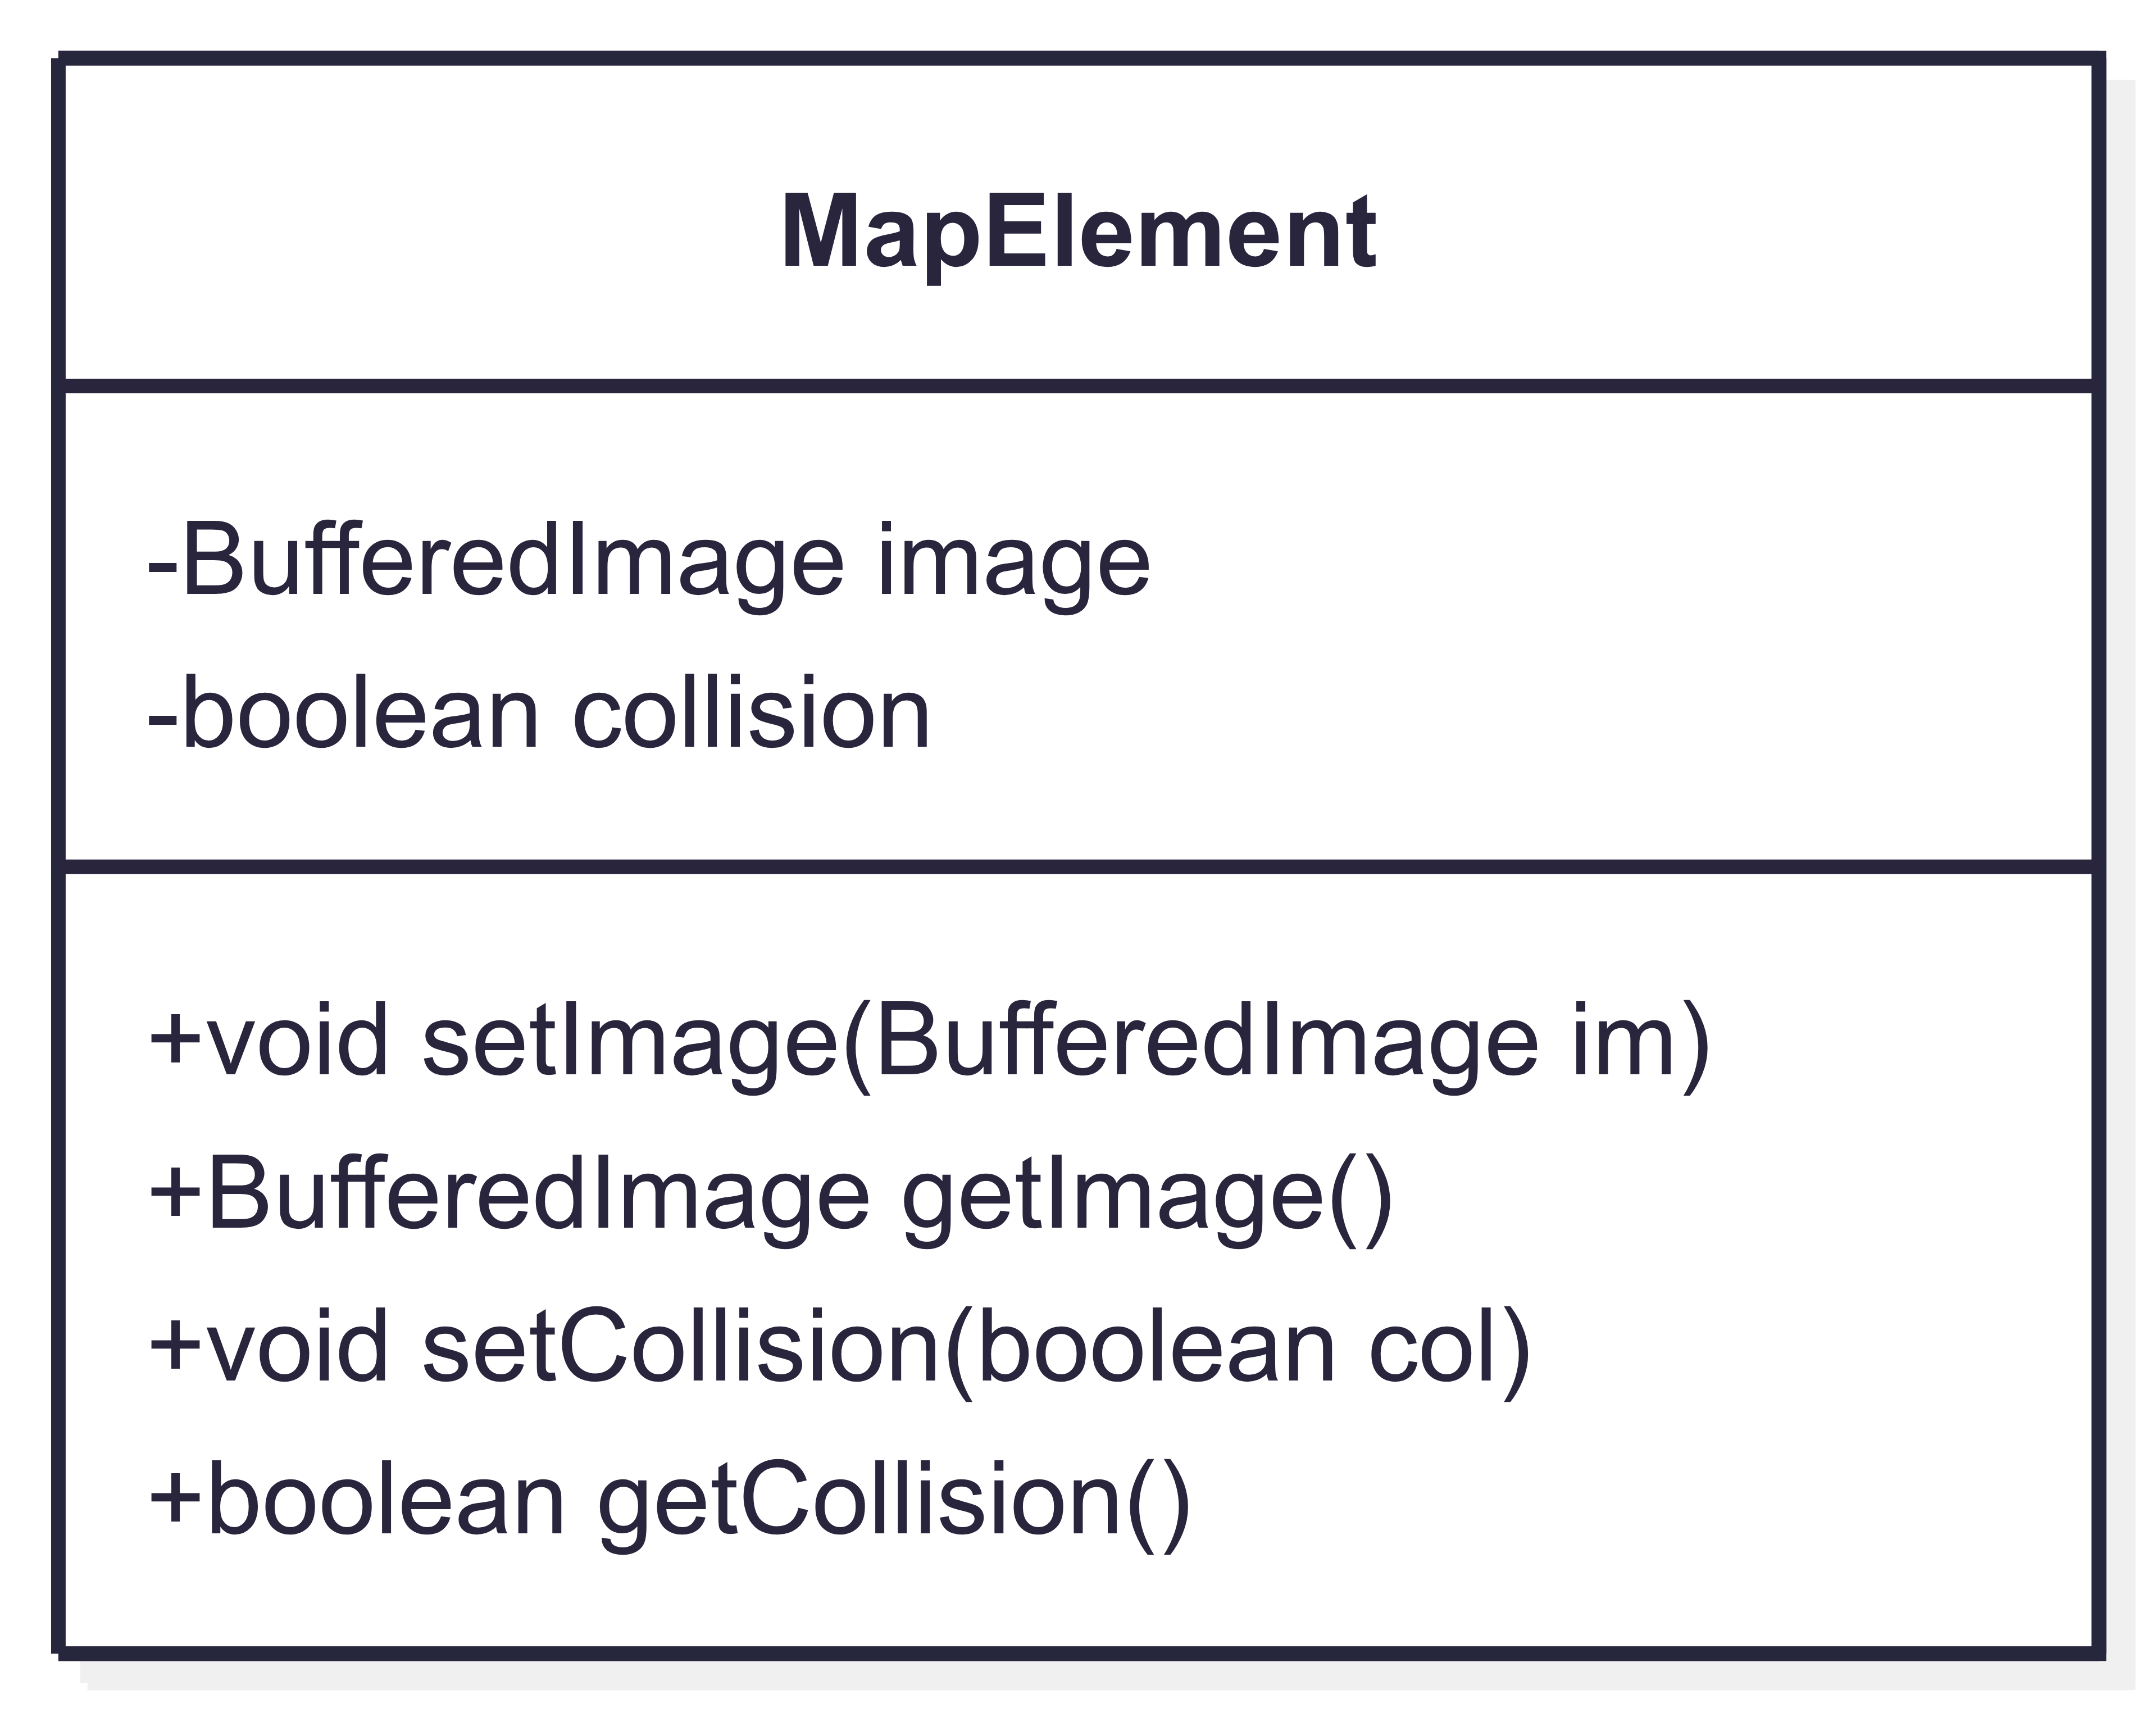
\includegraphics[width=0.8\textwidth]{resources/UMLMapElement.png}
    \caption{UML della classe MapElement nel model}
    \label{}
\end{figure}
Il pattern utilizzato è stato Immutable Object, un idioma fondamentale di OOP. Quest'ultimo spiega gli oggetti immutabili, oggetti che non
si possono veder modificato lo stato dopo la loro creazione. Sebbene gli oggetti nel progetto non siano perfettamente immutabili a causa
dei setter, quello a cui si aspirava era un oggetto non modificabile lontano da errori imprevedibili.
\section{Riccardo Cornacchia}
\section{Francesca Gatti}
\textbf{Problema}: Nel gioco è previsto un sistema di personalizzazione del personaggio tramite l'acquisto e la selezione di una nuova skin.
Il problema principale affrontato è stato quello di separare la gestione della parte logica del negozio, ovvero il controllo delle monete, 
delle skin e la selezione, dalla sua interfaccia grafica, mantenendo la possibilità di modificarlo in futuro.
\textbf{Soluzione}: Per affrontare questo problema è stato adottato il pattern Model-View-Controller (MVC), suddividendo le responsabilità 
tra i tre livelli:
\begin{itemize}
    \item Model: rappresentato dalla classe Shop, gestisce le skin disponibili, quella selezionata e lo stato di sblocco della skin (unlock). 
    Nel model sono inoltre presenti le due classi Skin e Score che permettono la gestione degli oggetti skin e punteggio da parte dello Shop.
    \item View: la classe ShopView è responsabile della visualizzazione delle informazioni (monete, stato skin) e della gestione dei pulsanti 
    che consentono l'acquisto e la selezione della nuova skin. L'utente è messo al corrente delle azioni che può fare nello shop grazie a 
    messaggi di dialogo che appaiono una volta cliccato il pulsante desiderato.
    \item Controller: ho implementato l'interfaccia ShopController che è responsabile della logica legata all'acquisto e alla selezione 
    delle skin e all'acquisizione dei dati e delle informazioni richieste dalla View. Inizialmente avevo implementato un'unica classe 
    all'interno del Model (la classe Shop), ma il codice risultava molto pesante e difficile da gestire.
\end{itemize}
L'introduzione del pattern MVC ha permesso di ottenere una struttura più chiara, estendibile e orientata al riuso.
\begin{figure}
    \centering
    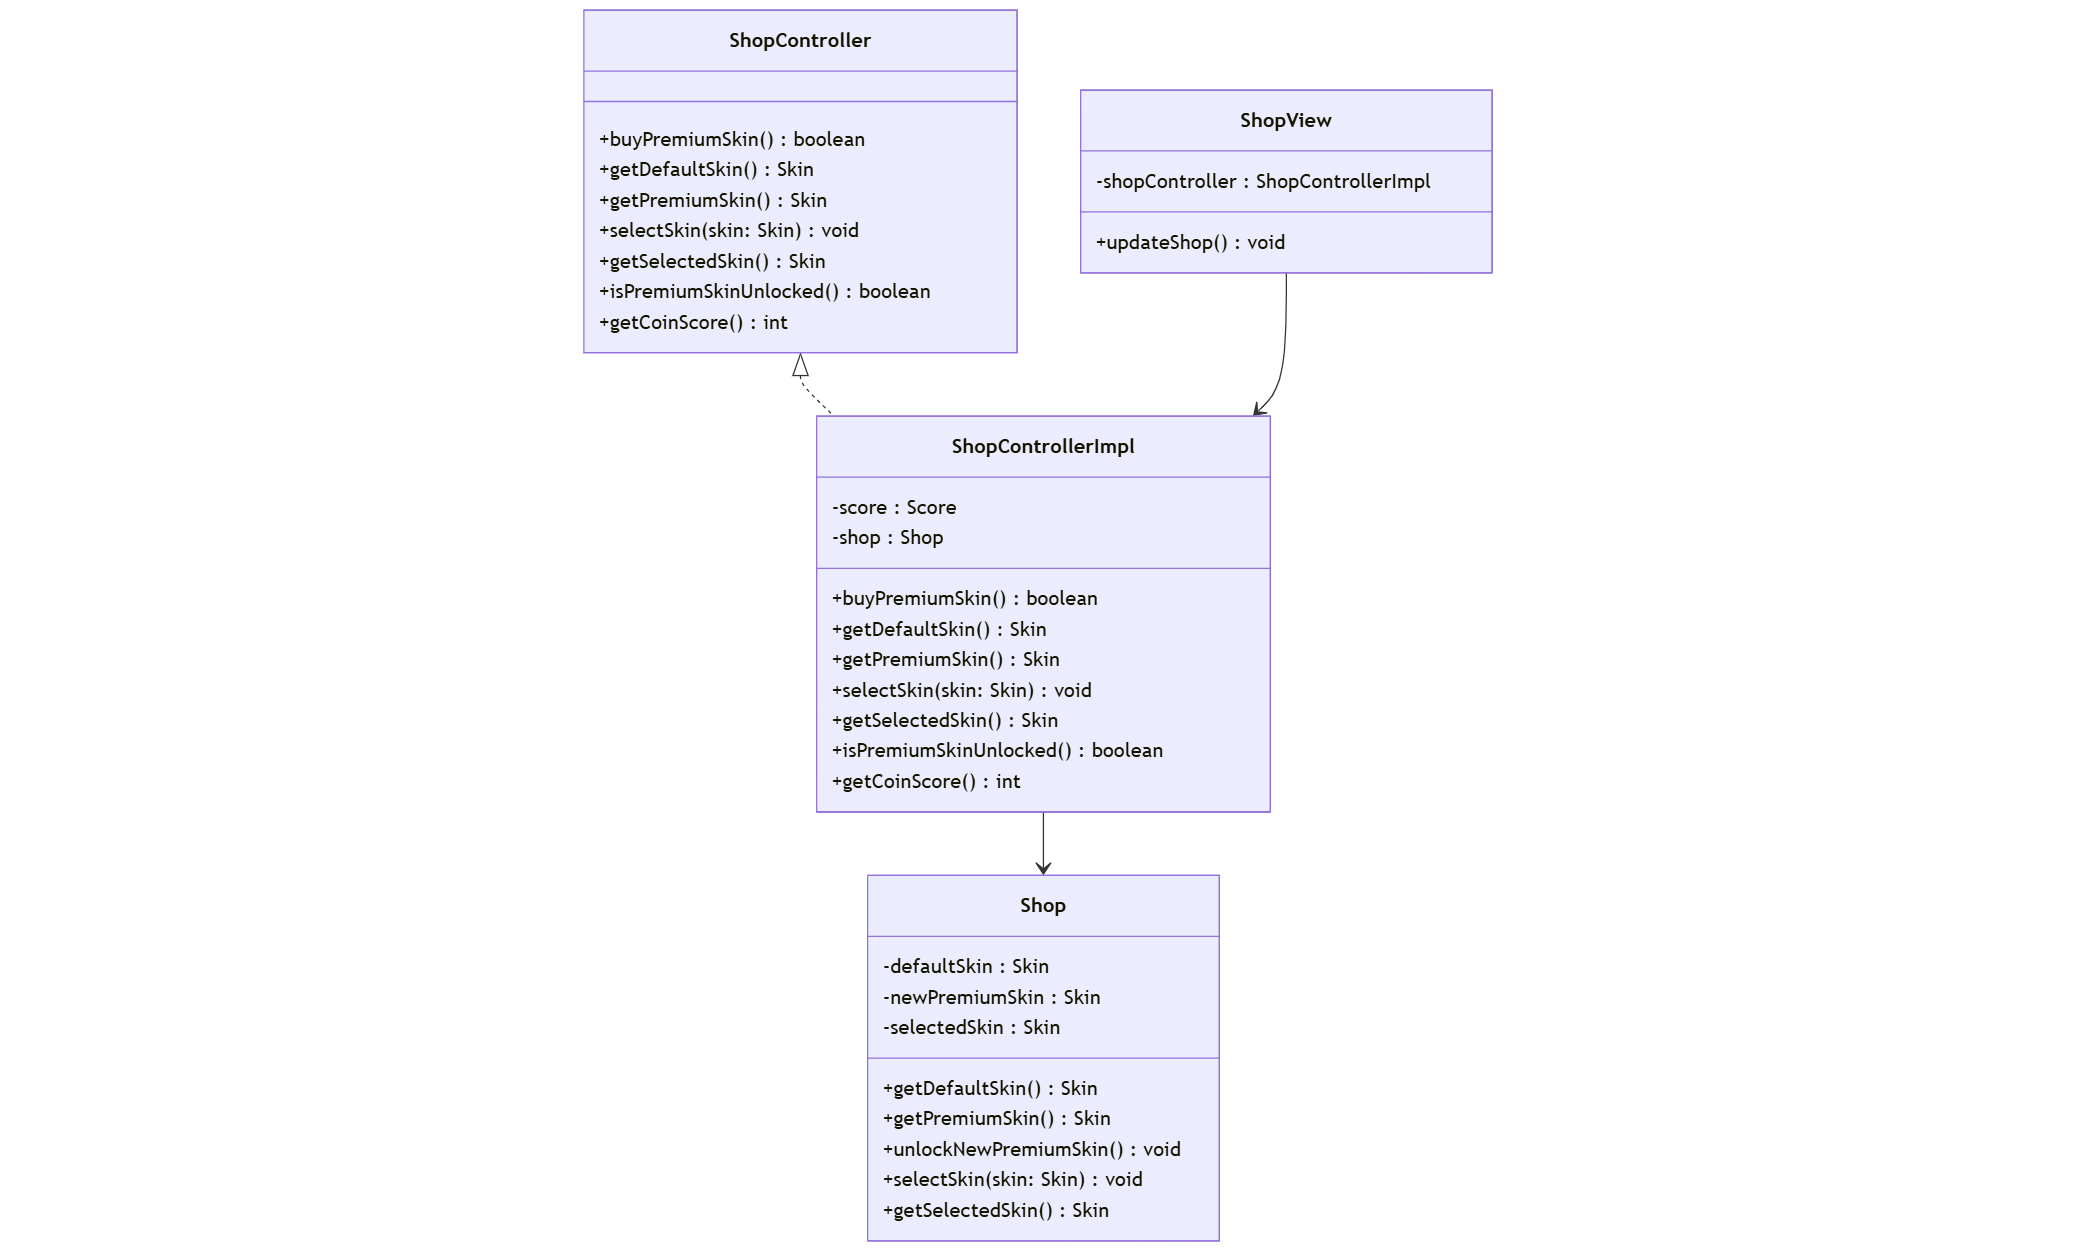
\includegraphics[width=0.8\textwidth]{resources/UMLshopMVC.png}
    \caption{UML dell'MVC per la gestione dello shop}
    \label{}
\end{figure}
\section{Giovanni Maria Rava}
\textbf{Problema:} I nemici del gioco devono muoversi da soli, invertire direzione appena urtano un ostacolo e restare sincronizzati con 
lo scorrimento della camera. 

\textbf{Soluzione:} Per gestire il movimento autonomo dei nemici e l'inversione di marcia in presenza di ostacoli ho adottato 
il pattern \emph{Model‑View‑Controller}. Il controller centrale è l'\emph{EnemyHandler}, che a ogni ciclo di gioco scorre l'intera lista di 
nemici: per ciascuno aggiorna prima lo stato logico delegando questa responsabilità all'oggetto model, \emph{EnemyImpl}, poi ne richiede 
la rappresentazione grafica all'oggetto view specifico, (ad esempio \emph{GoblinView}), per farla disegnare sul pannello di gioco. In questo modo 
la logica di collisione con la mappa e la scelta del momento in cui invertire la direzione restano incapsulate nel model, 
mentre il caricamento e il rendering rimangono confinati nella view; il controller non conosce i dettagli interni di nessuna delle due parti, 
ma si limita a coordinarne l'interazione. 
Questo assetto garantisce un codice più estendibile e manutenibile: introdurre una nuova tipologia di nemico richiede soltanto 
di aggiungere una nuova View, senza toccare il controller, e ogni modifica grafica o comportamentale resta circoscritta al relativo livello dell'architettura.
\begin{figure}
    \centering
    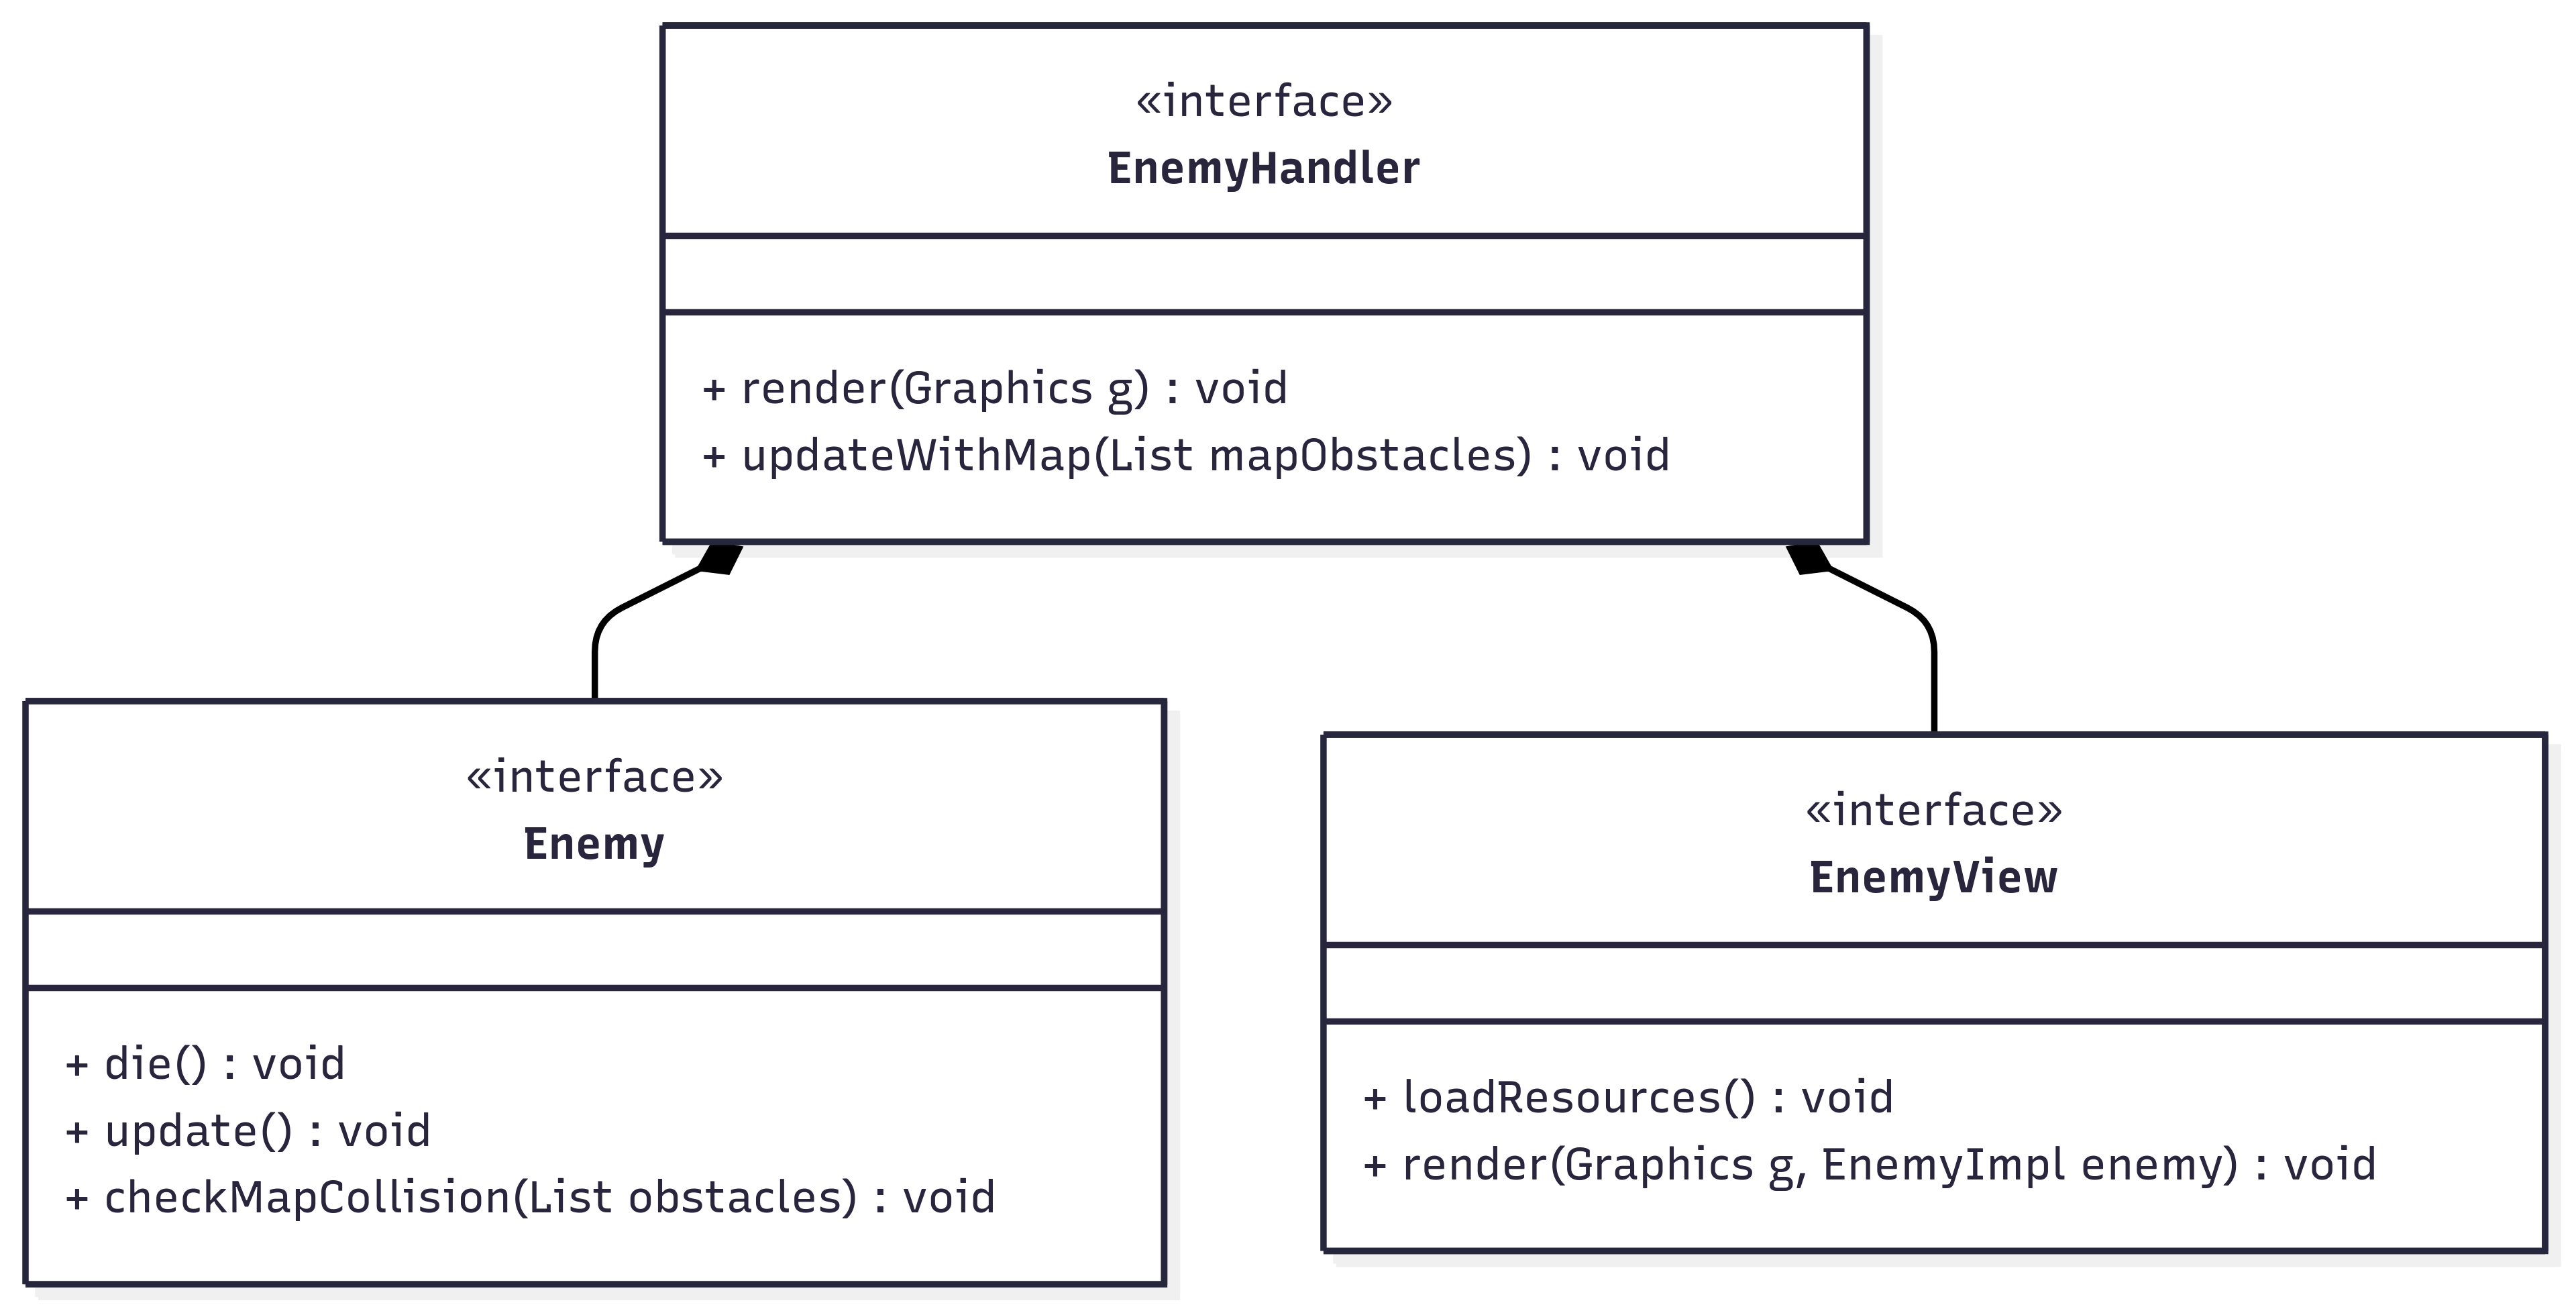
\includegraphics[width=0.8\textwidth]{resources/enemyMvcUml.png}
    \caption{UML dell'MVC per la gestione dei nemici}
    \label{}
\end{figure}
\newpage
\textbf{Problema:} Gestione il salvataggio del gioco e del caricamento del salvataggio all'apertura del gioco.\\
\textbf{Soluzione:} Il salvataggio e il ripristino della partita sono gestiti da un'unica classe, GameSaveManager, progettata come singleton 
per garantire un punto di accesso centralizzato e soprattutto per mantenere una unica istanza del file. Per rendere effettivo ciò,
all'interno della classe viene quindi eseguito un controllo specifico, in modo da non creare più file di salvataggio.
Quando il giocatore conclude un livello o chiude l'applicazione, i controller, \emph{ScoreController} e \emph{CoinController} invocano i relativi metodi 
per modificare le variabili e salvare lo stato di gioco, che si compone di:
\begin{itemize}
    \item Un intero che indica i livelli completati.
    \item Un intero che indica lemonete raccolte.
    \item Un booleano che indica l'acquisto della skin secondaria.
    \item Una stringa che indica la skin scelta.
\end{itemize}
All'avvio successivo, lo stato viene ricostruito e propagato ai vari model che lo necessitano; in caso contrario viene generata una partita nuova con parametri standard. 
L'intera logica di I/O è dunque isolata in una sola classe, priva di dipendenze dal motore di gioco; Questa architettura rende effettivo
il singleton e semplifica i test automatizzati.
\begin{figure}
    \centering
    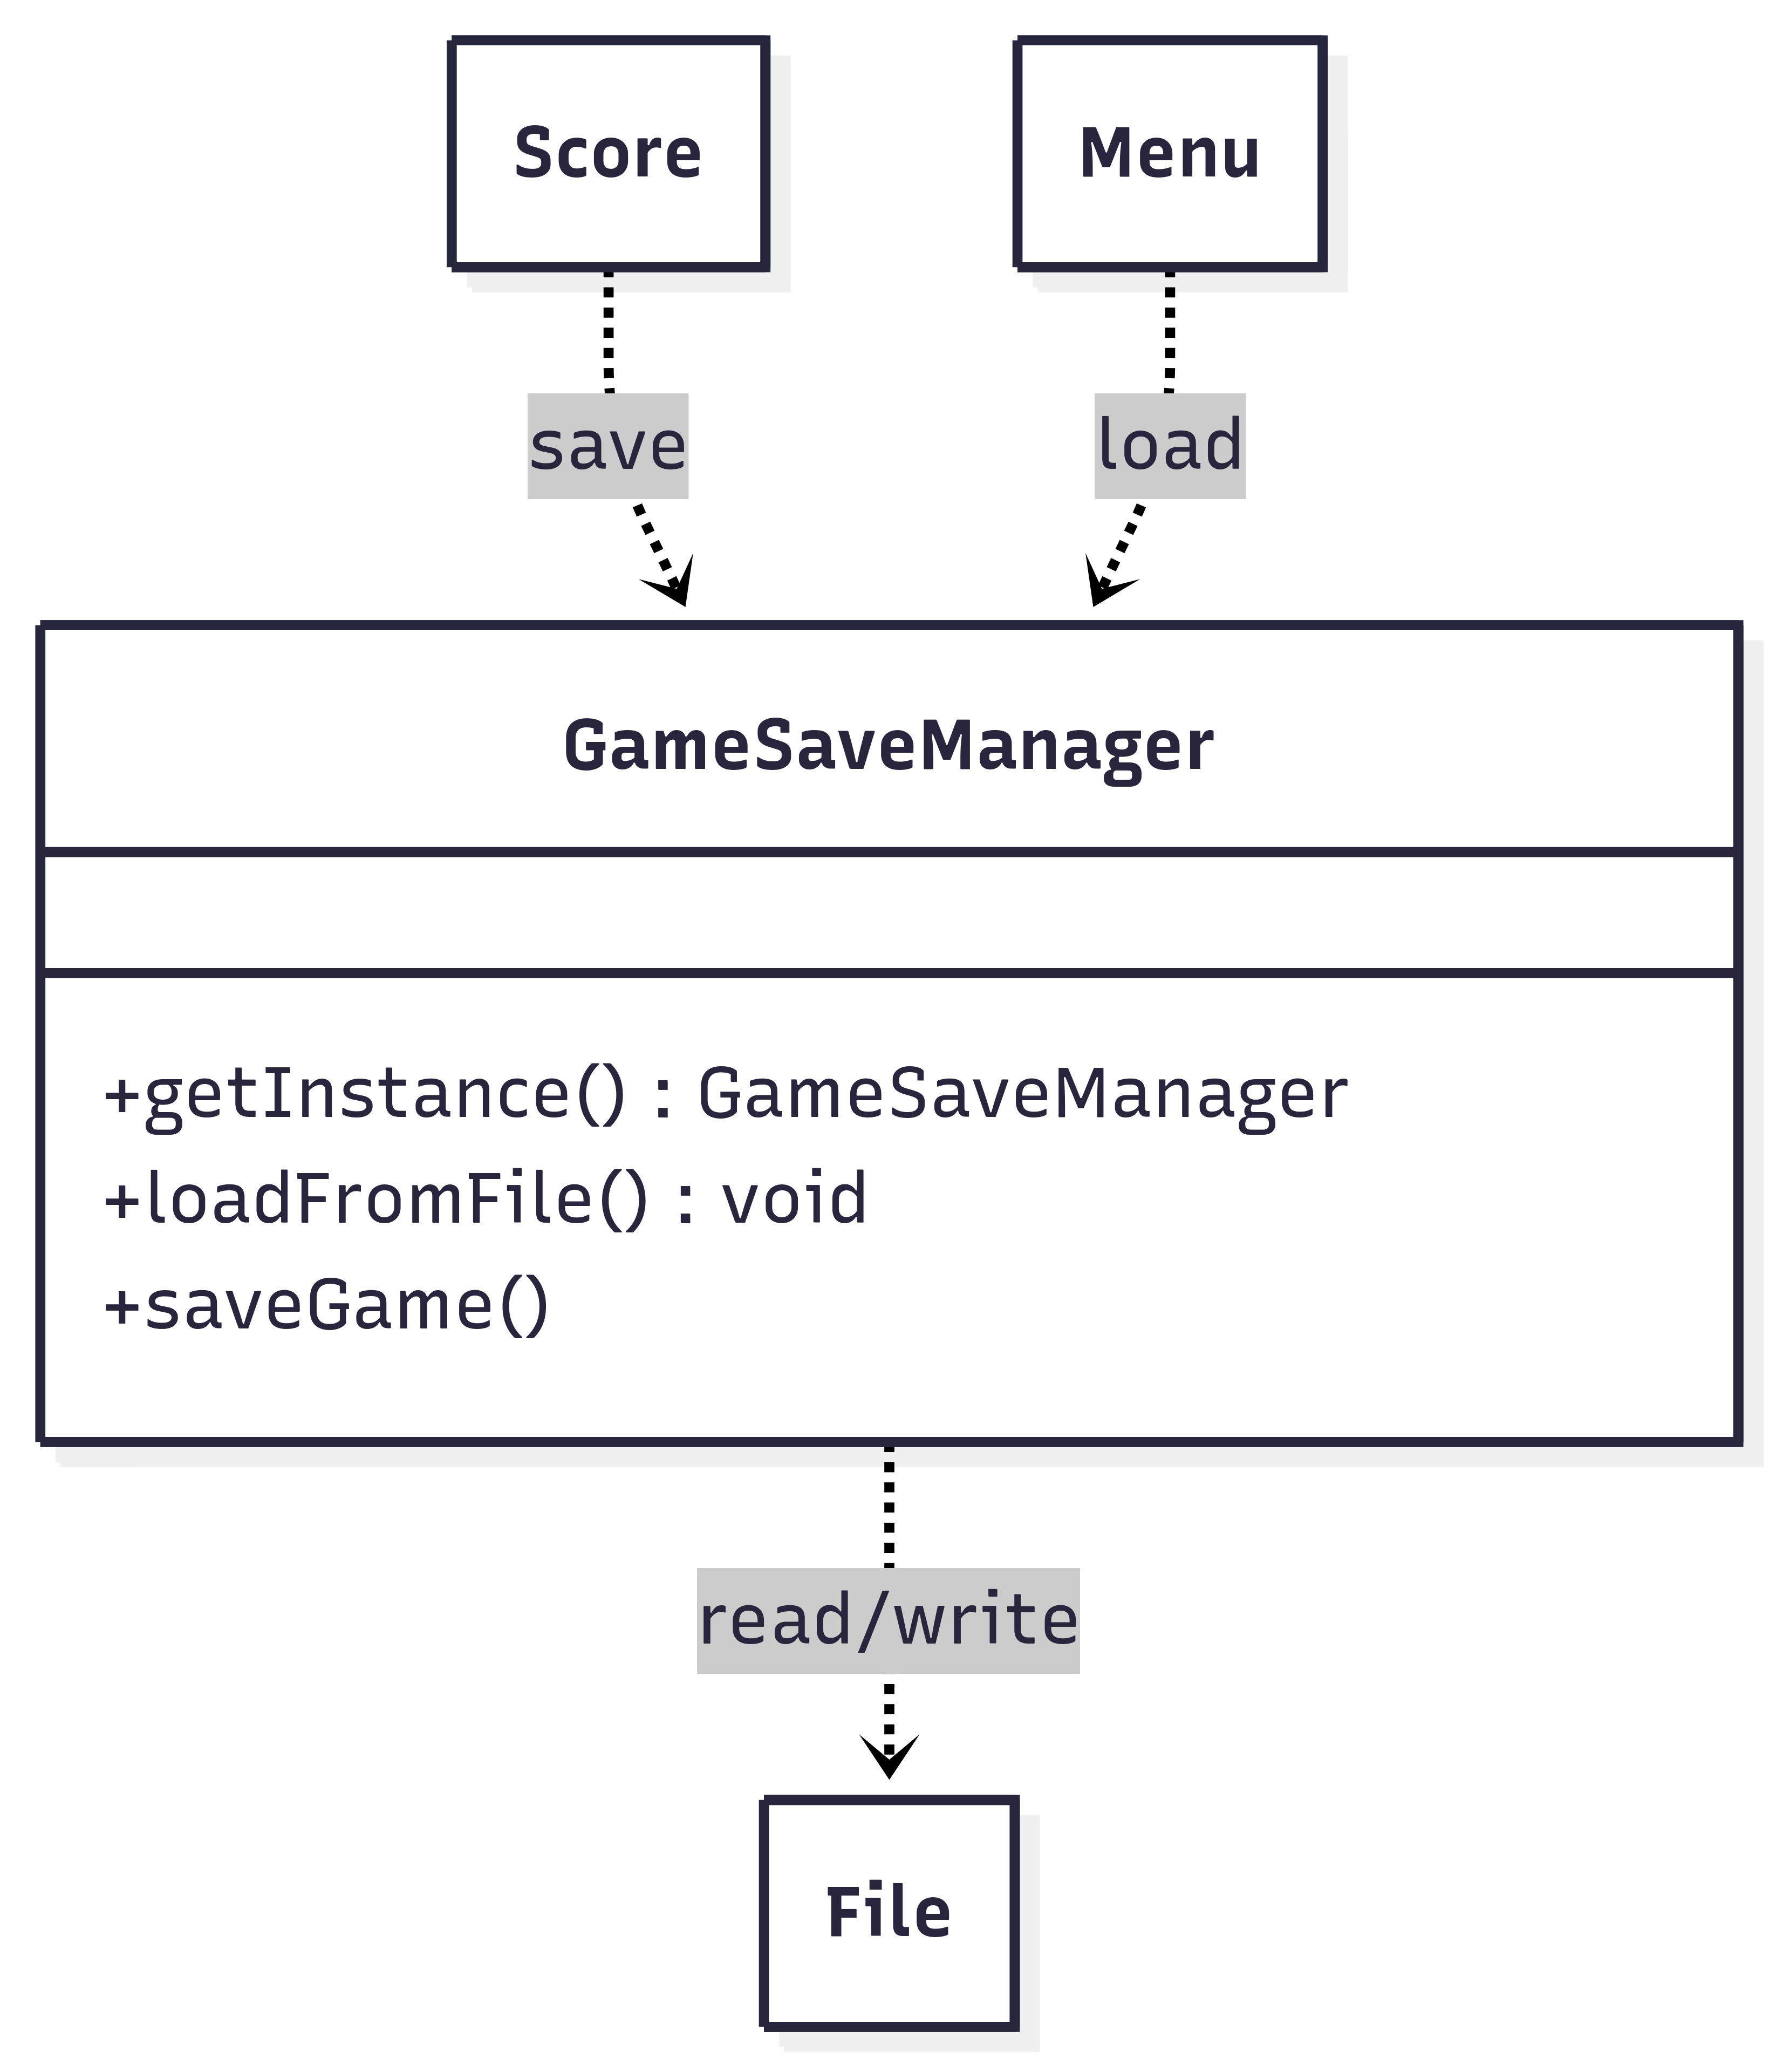
\includegraphics[width=0.8\textwidth]{resources/saveManagerUML.png}
    \caption{UML dell'MVC per la gestione dei nemici}
    \label{}
\end{figure}
\textbf{Problema} Nel livello di gioco occorre generare molti nemici in posizioni predefinite: ognuno deve comparire al momento giusto,
nella coordinata corretta e con la propria grafica, ma senza mescolare la logica di lettura dei dati con la scelta delle view. 

\textbf{Soluzione:} Il file \emph{enemies*.txt}, letto da EnemySpawner, elenca riga per riga tipo di nemico e coordinate. 
Ogni riga viene trasformata in un oggetto immutabile EnemySpawnPoints, che serve come contenitore dei dati di spawn. Durante 
l'esecuzione EnemySpawner rimane in ascolto dello scorrimento della mappa di gioco: quando un punto di spawn entra nell'area visibile, 
istanzia il relativo modello di nemico e, anziché occuparsi direttamente della grafica, delega la creazione della vista a EnemyViewFactory. 
Quest'ultima contiene un metodo che riceve l'identificativo numerico del nemico e restituisce la classe di rendering adeguata; 
la sua implementazione concreta, EnemyViewFactoryImpl, contiene la mappatura fra tipologia e view corrispondente (as esempio 1 $\rightarrow$ GuardView).
In questo modo la lettura del file, la gestione della memoria e il caricamento delle immagini restano ben separati: per aggiungere un 
nuovo tipo di nemico è sufficiente aggiungere una riga al file di mappa e una voce nella factory, senza toccare né il game‑loop né lo 
spawner, mantenendo il sistema estendibile e pulito.
\begin{figure}
    \centering
    \includegraphics*[width=0.8\textwidth]{resources/spawingEnemyUML.png}
    \caption{UML gestione spawing nemici}
    \label{}
\end{figure}
\chapter{Sviluppo}
\section{Testing automatizzato}
\end{document}